\documentclass{article}
\usepackage{times}
\usepackage{amssymb}
\usepackage{amsmath}
\usepackage{amsthm}
\usepackage{amsxtra}
\usepackage{algorithm}
\usepackage{algpseudocode}
\usepackage{color}
\usepackage{listings}
\usepackage{graphicx}

\newtheorem{theorem}{Theorem}

\newtheorem{myexample}{\textbf{Example}}
\newtheorem{mylemma}{\textbf{Lemma}}
\newtheorem{myproof}{\textbf{Proof}}
\newtheorem{myinvariant}{\textbf{Invariant}}
\newtheorem{mytheorem}{\textbf{Theorem}}
\newtheorem{mycorollary}{\textbf{Corollary}}
\newtheorem{myapproach}{Approach}
\newtheorem{myproperty}{Property}
\newtheorem{mydefinition}{Definition}
\newtheorem{myassumption}{Assumption}

\newtheorem{mycase}{Case}

\lstset{ %
  backgroundcolor=\color{white},   % choose the background color; you must add \usepackage{color} or \usepackage{xcolor}
  basicstyle=\footnotesize,        % the size of the fonts that are used for the code
  breakatwhitespace=false,         % sets if automatic breaks should only happen at whitespace
  breaklines=true,                 % sets automatic line breaking
  captionpos=b,                    % sets the caption-position to bottom
  commentstyle=\color{mygreen},    % comment style
  deletekeywords={...},            % if you want to delete keywords from the given language
  escapeinside={\%*}{*)},          % if you want to add LaTeX within your code
  extendedchars=true,              % lets you use non-ASCII characters; for 8-bits encodings only, does not work with UTF-8
  frame=single,                    % adds a frame around the code
  keepspaces=true,                 % keeps spaces in text, useful for keeping indentation of code (possibly needs columns=flexible)
  keywordstyle=\color{blue},       % keyword style
  language=Octave,                 % the language of the code
  morekeywords={assign, increment, decrement, jump, jump_if, store, *, +},            % if you want to add more keywords to the set
  numbers=left,                    % where to put the line-numbers; possible values are (none, left, right)
  numbersep=5pt,                   % how far the line-numbers are from the code
  rulecolor=\color{black},         % if not set, the frame-color may be changed on line-breaks within not-black text (e.g. comments (green here))
  showspaces=false,                % show spaces everywhere adding particular underscores; it overrides 'showstringspaces'
  showstringspaces=false,          % underline spaces within strings only
  showtabs=false,                  % show tabs within strings adding particular underscores
  stepnumber=1,                    % the step between two line-numbers. If it's 1, each line will be numbered
  stringstyle=\color{red},     % string literal style
  tabsize=2,                       % sets default tabsize to 2 spaces
  title=\lstname                   % show the filename of files included with \lstinputlisting; also try caption instead of title
}


\title{Algorithms and Data Structures}

\begin{document}

\maketitle

\section{Stable Matching}

Discussed by Gale, Shapley in 1962 (context of job markets): This problem is also related the allocation of workers in hospitals.

Each company a strict preference over applicants. Applicant has a strict preference over companies.

Is there a solution that is self-enforcing?

\begin{mydefinition}[Self-enforcing]
A matching is self-enforcing if for every applicant A and company C, such that A is not assigned to C, either:
\begin{itemize}
\item C prefers every one of its accepted applicants over A, or 
\item A prefers his current situation over working for C.
\end{itemize}
\end{mydefinition}



\section{Formal Model}

\begin{itemize}
\item Set X of man, 	$n = |X|$

\item Set Y of woman,	$m = |Y|$

\item Each $x \in X$ has a strict preference order $>_x$ over $Y$.

\item Each $y \in Y$ has a strict preference order $>_y$ over $X$.

\item Matching $M \subseteq X \times Y$ is a set of ordered pairs such that
every agent appears in at most one pair.
\end{itemize}

A blocking pair $(x,y)$ is a pair such that either $x$ or $y$ prefers some other person than its current match. A stable matching does not have blocking pairs.

\textbf{Problem:} Does there always exist a stable matching? Can we compute it in polynomial time?

Note: There may be solutions that are unfair, that is, they satisfy only one side (companies or workers).

\section{Deferred Acceptance Algorithm}

\textbf{Main idea}: Starts with an empty set of edges.

\begin{algorithmic}[1]
    \State{Initially, all $x \in X$ and all $y \in Y$ are free.}
    \While{$\exists$ free man $x$ that has not proposed to all women}
        \State{Let $y$ be the highest-ranked proposed women for $x$ that he hasn't proposed to
}
        \State{$x$ proposes to $y$}
        \If{$y$ is free}
            \State{$(x,y)$ gets engaged}
        \Else
            \State{$y$ currently engaged to $x'$}
            \If{$x >_y x'$}
                \State{$(x,y)$ gets engaged and $x'$ becomes free}
            \EndIf
        \EndIf
    \EndWhile
\end{algorithmic}

\begin{theorem}
The DA algorithm terminates after $n \cdot m$ iterations.
\end{theorem}
\begin{proof}
Some straightforward properties:
\begin{enumerate}
\item If $y$ becomes engaged, she will be matched in the end. The engagement partners are improving with respect to her preference $>_y$ over time.
\item $x$ proposes in decreasing order of $>_x$.
Thus, number of iterations is upper bounded by $n \cdot m$.
\end{enumerate}

Let $y >_x y'$ and $x >_y x'$. By contradiction, suppose in the final matching there is a BP, that is, we have a matching $M=\{(x,y'), (x', y)\}$.

- Note that $y >_x y'$, so by algorithm, $x$ proposed to $y$.

- Then $x$ proposed to $y'$, but $x$ becomes free afterwards.

- $y$ had a better engaged partner $x' >_y x$.

Contradiction.
\end{proof}

\subsection{Formalisms}

\begin{enumerate}

\item Woman $y$ is a \emph{valid partner} for a man $x$ if there exists a SM $M$ with $(x,y) \in M$.

\item Valid partner $y$ is the \emph{best valid partner} for man $x$ if for every valid partner $y' \neq y$, we have that $y >_x y'$.

\item Similar for \emph{worst valid partner}.
\end{enumerate}

\textbf{Notation:} $y = best(x)$ and $best(x) = x$ if $x$ has no valid partner.

We define the optimal matching as follows:

$$M^+ = \{ (x, best(x) | x \in X \wedge best(x) \neq x\}$$

\begin{theorem}
Every execution of the DA algorithm results in $M^+$.
\end{theorem}
\begin{proof}
Contradiction. Assume there is an execution $E$ of the DA algorithm resulting in a SM $M$, where some man is not matched to his best valid partner. This means that this man was rejected by a better valid partner during $E$.

Consider the first time that this happens, i.e., a man $x$ is rejected by a valid partner.

We have $(x',y)$, with $x' >_y x$.

\begin{enumerate}
\item $x$ proposed in decreasing order of preference, $y$ is ${best}(x)$.
\item $y$ rejects $x$, so $y$ is engaged to $x'$, with $x' >_y x$.
\item There exists Sm M with $(x,y) \in M$. Let $(x', y') \in M$.
\item Since rejection by $y$ was first in $E$, then $x'$ is not rejected by any valid partner when engaged to $y$. Since $y'$ is a valid partner of $x'$, $y >_x y'$. Then $(x', y)$ is a BP for $M$. But we assumed that $M$ is stable! Contradiction.
\end{enumerate}
\end{proof}

\begin{theorem}
In $M^+$, every woman is matched to her worst valid partner (if any).
\end{theorem}
\begin{proof}
Suppose $(x,y) \in M^+$ such that $x$ is not the worst valid partner of $y$.
Then there exists an SM $M'$ with $(x', y) \in M'$ and $x >_y x'$.
In $M'$ we have $(x, y') \in M'$. $y = {best}(x)$ and $y'$ is a valid partner for $x$. So $y >_x y'$. Then $(x,y)$ is a BP in $M'$. Contradiction.
Similar if $x$ is unmatched in $M'$.
\end{proof}

\newpage

\section{Prerequisites}

\begin{itemize}

\item \textbf{Algorithm:} A step-by-step procedure for solving a certain \emph{problem}, e.g., ``sorting $n$ numbers'', ``find the closest coffee shop to your position''.

\item \textbf{Quality Criteria:} termination,  correctness, speed, memory, simplicity, generality, randomization, approximation Quality.

\item \textbf{Data Structure:} An organization of data such that certain operations can be handled efficiently. Ex: lists, heaps, etc.

\item \textbf{Quality Criteria:} memory, preprocessing time, query time, update time, simplicity

\end{itemize}

To evaluate the performance, we require a model.


\subsection{Random Access Model}

Memory consists of a sequence of cells, with an address ${addr} \in \mathbb{N}$. There are registers that can hold data, where operations may be performed. We assume the word size if polynomially bounded in $\log n$.

In this model, an algorithm is a numbered sequence of basic operations. The input of size $m$ for the algorithm is stored in memory $\{0, \ldots, m-1\}$. We have the following basic operations:

\begin{enumerate}
\item \textbf{load($i$, $j$):} Loads the content the memory cell with address stored in register $i$ into register $R_j$.
\item \textbf{store($i$, $j$):} Stores the content of register $i$ into the memory cell addressed by register $R_j$.
\item \textbf{assign($i$, $C$):} Stores $C$ into register $R_i$.
\item \textbf{increment/decrement($i$):} Increases/decreases value at $R_i$ by 1.
\item \textbf{op($i$, $j$, $k$):} Stores $R_i {op} R_j$ into $R_k$. ${op} \in \{+, \times, 0, \div, \mod, \wedge, \vee, \ldots\}$.
\item \textbf{jump($i$):} Jumps to operation $i$ in the algorithm.
\item \textbf{jump\_if($i$, $j$):} Jumps to operation $i$ in the algorithm if $R_j = 0$.
\end{enumerate}

\begin{algorithm}[h]
\begin{lstlisting}
assign(1, n) %*\quad*) -- 1
assign(2, 0) %*\quad*) -- 1
decrement(1) %*\quad*) -- n
load(1,3) %*\quad*) -- n
*(3,3,3) %*\quad*) -- n
+(3,2,2) %*\quad*) -- n
jump_if(8,1) %*\quad*) -- n
jump(2) %*\quad*) -- n-1
store(2,0) %*\quad*) -- 1
\end{lstlisting}
\caption{Add the squares of the first $n$ numbers in memory. The time complexity is $6n +2$.}
\end{algorithm}

\textbf{Cost Model}: Every basic operation takes one time unit to execute.

\begin{mydefinition}[Time Complexity]
The time complexity/runtime of algorithm $A$ for input $I$, $T_A(I)$, is the number of basic operations performed by $A$ on $I$.
\end{mydefinition}

With this definition of time complexity, we can compare speeds using natural functions.

\begin{mydefinition}[Worst-case]
The worst-case complexity $T_A^{wc}(n)$ of algorithm $A$ is equal to $\max\{I_A(I) | I \in I_n\}$.
\end{mydefinition}

\begin{mydefinition}[Best-case]
The best-case complexity $T_A^{wc}(n)$ of algorithm $A$ is equal to $\min\{I_A(I) | I \in I_n\}$.
\end{mydefinition}

\begin{mydefinition}[Average-case]
The average-case complexity $T_A^{wc}(n)$ of algorithm $A$ is equal to $\frac{1}{|I_n|} \sum\limits_{I \in I_N} T_A(I)$.
\end{mydefinition}

\subsection{O-notation}

\begin{mydefinition}
Let $f: \mathbb{N} \rightarrow \mathbb{R}_+$ be a function, then:

$$O(f(n)) = \{g: \mathbb{N}\rightarrow \mathbb{R}_+: \exists c>0, \exists n_0 \in \mathbb{N}, \forall n \ge n_0: g(n) \le c \cdot f(n)\}$$

$$\Omega(f(n)) = \{g: \mathbb{N}\rightarrow \mathbb{R}_+: \exists c>0, \exists n_0 \in \mathbb{N}, \forall n \ge n_0: g(n) \ge c \cdot f(n)\}$$

$$\Theta(f(n)) = O(f(n))\cap \Omega(f(n))$$

$$o(f(n)) = \{g: \mathbb{N}\rightarrow \mathbb{R}_+: \forall c>0, \exists n_0 \in \mathbb{N}, \forall n \ge n_0: g(n) \le c \cdot f(n)\}$$

$$\omega(f(n)) = \{g: \mathbb{N}\rightarrow \mathbb{R}_+: \forall c>0, \exists n_0 \in \mathbb{N}, \forall n \ge n_0: g(n) \ge c \cdot f(n)\}$$

\end{mydefinition}

Observation:
\begin{itemize}
\item $g \in O(f) \approx ``g \le f''$,
\item $g \in \Omega(f) \approx ``g \ge f''$,
\item $g \in \Theta(f) \approx ``g = f''$,
\item $g \in o(f) \approx ``g < f''$,
\item $g \in \omega(f) \approx ``g > f''$.
\end{itemize}

\begin{mylemma}
Let $p(n) = \sum\limits_{i=0}^k a_i \cdot n^i$ with $a_k > 0$. Then $p(n) \in \theta(n^k)$.
\end{mylemma}
\begin{proof}
\begin{enumerate}
\item (Show that $p \in O(n^k)$).

$$p(n) = \sum\limits_{i=0}^k a_i \cdot n^i \le \sum\limits_{i=0}^k |a_i| \cdot n^i
\le \sum\limits_{i=0}^k |a_i| \cdot n^k \le \left ( \sum\limits_{i=0}^k |a_i| \right )\cdot n^k \le c \cdot n^k$$

\item (Show that $p \in \Omega(n^k)$).

$$p(n) \ge a_k \cdot n^k - \sum\limits_{i=0}^{k-1} |a_i| \cdot n^i \ge
a_k \cdot n^k - n^{k-1} \cdot \sum\limits_{i=0}^{k-1} |a_i| =
\frac{a_k}{2} n^k +  \frac{a_k}{2} n^k - A \cdot n^{k-1} = \frac{a_k}{2} n^k + n^{k-1}(\frac{a_k}{2} n - A) \ge $$

\end{enumerate}
\end{proof}

\begin{mylemma}
If $L := \lim_{n \rightarrow \infty} \frac{f(n)}{g(n)}$ exists, then:

If $L = 0$ then $f(n) \in o(g(n))$. If $L \in (0, \infty)$ then $f(n) \in \Theta(g(n))$. If $L = \infty$ then $f(n) \in \omega(g(n))$.
\end{mylemma}
\begin{proof}
{\color{red} HOMEWORK!}
\end{proof}


\begin{mylemma}
$n \log(n) \in o(n^{1+\epsilon}$ for any $\epsilon > 0$.
\end{mylemma}
\begin{proof}
$\lim_{n \rightarrow \infty} \frac{n \log n}{n^{1+\epsilon}} =
\lim_{n \rightarrow \infty} \frac{\log n}{n^{\epsilon}} =
\lim_{n \rightarrow \infty} \frac{\frac{1}{n}}{\epsilon \cdot n^{\epsilon - 1}} =
\lim_{n \rightarrow \infty} \frac{1}{\epsilon \cdot n^{\epsilon}} = 0.$
\end{proof}

\begin{algorithm}
\begin{lstlisting}
Bubble_sort()
Input: a[1], ..., a[n]
Output: Sorted sequence
For i from 1 to n-1 do
    max_index = i
    For j from i+1 to n do
        if a[j] > a[max_index]
        then max_index = j
    end do
    if i != max_index then
        swap(a[i], a[max_index])
end do
\end{lstlisting}
\end{algorithm}

We compile this pseudocode to the machine model. This leads to the following cost model:

\begin{itemize}
\item cost(basic operation) = 1
\item cost(\textbf{if} A \textbf{then} B \textbf{else} C) = cost (A) + max\{cost(B), cost(C)\}
\item cost(\textbf{while} A \textbf{do} B) = (cost(A) + cost(B)) $\cdot$ iterations of the loop
\end{itemize}

Example. The cost of Bubble Sort is:

\begin{align*}
&\sum\limits_{i=0}^{n-1} (1 + (\sum\limits_{j=i+1}^n 3) + 3) = \sum\limits_{i=0}^{n-1} 4 + 3 \cdot \sum\limits_{j=i+1}^n 3 = \\
&= 4n + 3 \sum\limits_{i=0}^{n-1} (n-i) = 4n + 3 \sum\limits_{i=1}^{n} i = \ldots = \Theta(n^2) \\
\end{align*}


\section{Basic Data Structures}

\noindent \textbf{Goal:} Store ordered sequences $a_1, \ldots, a_k$ of elements.

\subsection{(Static) Array}

We can store elements in a contiguous region of memory. Element $a_i$ can be accessed in constant time.

\begin{itemize}
\item \textbf{(+)} Access to $i^{th}$ element
\item \textbf{(-)} Insert, delete
\end{itemize}

\subsection{Linked Lists}

\noindent Each \emph{item} contains:
\begin{enumerate}
\item An element $e$
\item Pointer to next item in the sequence
\item Pointer to the previous item in the sequence
\end{enumerate}

\noindent We also allocate a \emph{dummy item/head} that contains:
\begin{enumerate}
\item Stores $\bot$ (\emph{nil})
\item Next pointer points to first element
\item Prev pointer points to last elements
\end{enumerate}

A pointer to the \emph{head} item is used as a starting point for the operations (passed by parameter). We have the following operations:

\begin{itemize}
\item \emph{first\_element(h), last\_element(h), is\_empty(h)}: $\Theta(1)$
\item \emph{splice(a,b,t)}: Cuts entire sub-list $[a,b]$ and puts it between $t$ and $t'$. $\Theta(1)$
\item \emph{insert\_after(v, a)}: Takes element $v$ and inserts it after $a$. $\Theta(1)$
\item \emph{remove(a)}: Removes $a$ from its list. $\Theta(1)$
\item \emph{size of list}: It depends, since elements of sublists cannot be easily counted!
\item \emph{find(h, x)}: Is $x$ an element of the list? Returns pointer to the item that contains $x$, or $h$ if $x \notin $ list.
\end{itemize}

\begin{algorithm}
\begin{lstlisting}
insert_after(v,a):
    Create a list L with one item i, storing v.
    splice(v, v, a)
    Delete L.
\end{lstlisting}
\begin{lstlisting}
remove(a):
    Create empty list L with head h.
    splice(a, a, h)
    Delete L.
\end{lstlisting}
\begin{lstlisting}[mathescape]
find1(h,x):
    cur $\gets$ h->next
    while cur->e != x do
        if (run ==h) then break
        run $\gets$ cur->next
    end do
    return cur
\end{lstlisting}
\begin{lstlisting}[mathescape]
find2(h,x) [Sentinel Search]:
    (h->e) $\gets$ x
    cur $\gets$ h->next
    while cur->e != x do
        cur $\gets$ cur->next
    end do
    h->e $\gets \bot$
    return cur
\end{lstlisting}
\end{algorithm}

\newpage

\subsection{Unbounded Arrays}

We want to support
\begin{itemize}
\item Operator []: quick access to $i^{th}$ element
\item push\_back(v): append v to array
\item pop\_back(): Remove last element
\item size(): Returns number of elements
\end{itemize}

\noindent \textbf{Idea:} Static array of size $w$ for storing $n$ elements, with $w \ge n$. To fix the problem of having a limited array, we do a reallocation. We move all elements to a new array that is twice as large. Whenever $n \le \frac{w}{4}$ starts to be the common case, we reallocate the array to half size.

The problem is that push and pop can take:
\begin{itemize}
\item $\Theta(1)$ if no alloc is needed (good case)
\item $\Theta(n)$ if alloc is needed (bad case)
\end{itemize}

However, a bad case is preceded by roughly $n$ good cases to happen. In other words, the bad case is amortized by the good case. The following lemma shows that push-/pop-back operations have constant \emph{amortized} worst-case complexity.

\begin{mylemma}
A sequence of $m$ push-/pop-backs takes $\Theta(m)$ time.
\end{mylemma}
\begin{proof}[Proof (Bank Account Method)]
For any push-back we pay 2 tokens to a bank account. For any pop-back, we pay 1 token. We show that for a reallocation, we have enough tokens on the account to pay for moving the elements.

By induction. We initialize an empty array with $w=1$. $a_0$ adds 2. For the first reallocation, we have enough tokens to pay for the move.

After a reallocation, it holds that $n = w/2$. The next reallocation happens if (1) $n = w$ or if $n = w/4$. If $n=w$, we must have performed $w/2$ push-backs.
So, the bank account has at least $w$ tokens. enough for the $w$ movesin the next reallocation. If $n = w/4$, then we have $w/4$ pop-backs, each paying 1 token. So, the bank account has at least $w/4$ tokens. That is enough to pay for the move.
\end{proof}

\newpage

\subsection{Stacks, Queues, Deques}

\noindent Stacks support:
\begin{itemize}
\item push\_back(v)
\item pop\_back()
\item last()
\item size()
\end{itemize}

\noindent Queues support:
\begin{itemize}
\item push\_back(v)
\item pop\_front()
\item first()
\item size()
\end{itemize}

\noindent Queues support:
\begin{itemize}
\item push\_back(v)/push\_front(v)
\item pop\_front()/pop\_front()
\item first()/last()
\item size()
\end{itemize}

\noindent Lists (with restricted splice) can do all that in $\Theta(1)$.

\bigskip \noindent Stacks can be implemented with unbounded arrays.

\bigskip \noindent Queues can be implemented with circular arrays of fixed size $w$, using two pointers \emph{head} and \emph{tail}. Range $[h, t-1]$ stores the entries. Array is empty if $h = t$, and the size $n$ is given by $n = (t - h + w) \mod w$. We do reallocation as usual, by checking the size. This also works for deques.

\subsection{Basic Probability}

\textbf{Probability space $S$}: finite set with probabilities $P_s$ for $s \in S$, such that ${\sum_{s \in S} P_s = 1}$.

\noindent \textbf{Uniform probability space:} S is uniform if $\forall s \in S, P_s = 1/|S|$.

\noindent \textbf{Event:} $E \subseteq S$. ${prob}(E) \triangleq \sum_{S \in E} P_S$. If $S$ is uniform, ${prob}(E) = \frac{|E|}{|S|}$.

\noindent \textbf{Random Variables:} $X: S \rightarrow \mathbb{R}$
\begin{itemize}
\item can be composed: $X+Y, X\cdot Y, \ldots$
\item can be used for events: ${prob}(X \ge 5)$
\item indicator variables: $X: S \rightarrow \{0, 1\}$
\end{itemize}

\noindent \textbf{Expected Value:} $E[X] = \sum_{P_s X(s)} = \sum_{z \in \mathbb{R}} z \cdot {prob}(X = z)$.

\noindent \textbf{Linearity of expectation:} $E[X + Y] = E[X] + E[Y]$.

Variables $X_1,\ldots,X_k$ are independent if $\forall x_1,\ldots,x_k \in S$, ${prob}(X_1 = x_1 \wedge \cdots \wedge X_k = x_k) = \prod_{1 \le i \le k} {prob}(X_i = x_i)$.

\bigskip \noindent If $X$ and $Y$ are independent, then $E[X \cdot Y] = E[X] \cdot E[Y]$.

\bigskip \noindent \textbf{Markov Inequality:} For a non-negative $X$ and $x > 1$, ${prob}(X \ge k E[X]) \le 1/c$. 



\newpage

\section{Quicksort}

\begin{algorithm}
\begin{lstlisting}[mathescape]
quicksort($a_0\ldots a_{n-1}$)

    Choose pivot element $a_p$
    L $\gets$ ()
    H $\gets$ ()
    for $i=0,\ldots,n-1$ do
        if $a_i < a_p$ then $L \gets L . a_i$
        if $a_i > a_p$ then $H \gets L . a_i$
    end do
    return quicksort(l) . $a_p$ . quicksort(H)
\end{lstlisting}

\end{algorithm}

How to choose pivot?

\begin{enumerate}
\item Choose $p=0$?

$\Theta(n^2)$ runtime if list is already sorted. However, average case complexity is $\Theta(n \log n)$. But why should the input be uniformly distributed?

\item Choose $p \in \{0, \ldots, n-1\}$ uniformly at random (u.a.r.).

\begin{mytheorem}
The expected number of comparisons in quicksort is at most $2\cdot n \cdot \log n$ (for every input).
\end{mytheorem}
\begin{proof}
Let $a_0',\ldots,a_{n-1}'$ be the sorted sequence. Each pair is compared at most once. Define indicator variables

$X_{ij} = 1$ if $a_i'$ and $a_j'$ are compared.

$X_i = \sum_{i < j} X_{ij}$ is the number of comparisons.

We show that ${prob}(X_{ij} = 1) \le \frac{2}{j - i + 1}$. Consider $\{a_i', \ldots, a_j'\}$ and let $p$ be the first pivot chosen from $\{a_i', \ldots, a_j'\}$. We compare $a_i'$ and $a_j'$ iff $p \in \{a_i', a_j'\}$. The probability for that is 2 divided by the size of the list: $\frac{2}{j - i + 1}$.

\begin{align*}
E[X] = E[\sum X_{ij}] = \sum E[X_{ij}] \le \sum_{0 \le i < j \le n-1} \frac{2}{j - i + 1} \\
= \sum_{i = 0}^{n-2} \sum_{j= i+1}^{n-1} \frac{2}{j -i + 1} = 2 \sum_{i = 0}^{n-2} \sum_{k=2}^{n-i} \frac{1}{k} \le 2 \sum_{i = 0}^{n-2} \sum_{k=2}^{n} \frac{1}{k} \\
\le 2 n \cdot \ln n (\mbox{Because } \sum_{k=1}^n \frac{1}{k} \le \ln n + 1)
\end{align*}

\end{proof}

\end{enumerate}

\newpage

\section{Hashing}

\begin{itemize}
\item We want to represent a \emph{set} $S = \{e_1,\ldots,e_n\}$.
\item Each element $e$ has a key, ${key}(e) \in U$ (``universe'').
\end{itemize}

Assume that keys are pw distinct.

\subsection{Dictionary problem}

\begin{itemize}
\item insert(e, S)
\item remove(k, S) - remove element with key $k$ from $S$
\item search(k, S) - return element with key $k$ in $S$ or $\bot$
\end{itemize}

If $|U|$ is small, just use an array of size $|U|$. But we can instead use an array of size $m$, with $m \equiv n$.

\begin{mydefinition}
A hash function $h$ is a map $h: U \rightarrow \{0, \ldots, m-1\}$. We write $h(e) = h(key(e))$.
\end{mydefinition}

We want to put element $e$ at position $h(e)$ in array. But there may be a collision (because the function is non-injective).

\subsection{Chaining}

We add a linked list per cell.

\begin{itemize}
\item insert(e, S): push\_back in list, $\theta(1)$.
\item search(k, S): Scan through the appropriate list.
\item remove(k, S): Similar to search + removal from list.
\end{itemize}

What is the length of the lists? $\Theta(n)$ in the worst case.

\begin{mydefinition}
A family $H$ of hash functions is called \emph{c-universal} for $c \ge 1$, if for all $x,y\in U, |\{h\in H: h(x) = h(y)\}| \le \frac{c}{m} |H|$. That is, when choosing $h$ uniformly at random from $H$, ${prob}(h(x)=h(y)) \le \frac{c}{m}$.
\end{mydefinition}

\begin{myexample}
The family of all possible hash functions $U \rightarrow \{0, \ldots, m-1\}$ is 1-universal (but too large to be useful).
\end{myexample}

\noindent We assume that evaluating $h$ takes constant time.

\begin{mytheorem}
For hashing with chaining, using a c-universal family of hash functions, the expected cost of a search/remove operation is $O(1 + c \cdot \alpha)$, where
$\alpha = \frac{n}{m}$, the \emph{load factor} of the hash table.
\end{mytheorem}
\begin{proof}
Fix an element $\tilde{e}$ and $k = {key}(\tilde{e})$, and let $X$ be the length of the list at $h(k)$.

For $e \in S$, we set $X_e = 1$ if $h(e) = h(\tilde{e})$, and $X_e = 0$ otherwise.

$$E[X] = \sum_{e \in S} E[X_e] = \sum_{e \in S} {prob}(X_e=1) = \sum {prob}(h(e)=h(\tilde{e})) \le \sum_{e \in S} \frac{c}{m} = c \cdot \frac{n}{m} = c \alpha $$
\end{proof}

\subsection{Construction of a 1-universal family}

Assume $w = \lfloor \log_2 m \rfloor$. For $U = \{0, \ldots, u-1\}$, write $x \in U$.

\bigskip \noindent We split the string $x$ in w-bit strings $(X_1, X_2, X_3, \ldots, X_k)$.
Choose $k$ random numbers $a = (a_1, \ldots, a_k) \in \{0, \ldots, m-1\}^k$.

$$h_a(x) = \sum\limits_{i=1}^k a_i \cdot x_i (\mod m)$$

\begin{mytheorem}
$H = \{h_a | a \in \{0, \ldots, m-1\}^k\}$ is 1-universal if $m$ is a prime.
\end{mytheorem}
\begin{proof}
Consider $x,y \in U$ with $x \neq y$. W.l.o.g., assume $x_1 \neq y_1$. Now, fix $a_2,\ldots, a_k$ arbitrarily. Then,

\begin{align*}
h(x) = h(y) &\iff \sum\limits_{i=1}^k a_i x_i \equiv \sum\limits_{i=1}^k a_i y_i \mod m \\
& \iff a_1(x_1 - y_1) \equiv - \sum\limits_{i=2}^k a_i (x_i - y_i) \mod m \\
& \iff a_1 \equiv (x_1 - y_1)^{-1} \cdot (- \sum \ldots) \mod m
\end{align*}

There are $m^{k-1}$ choices for $a_2, \ldots, a_k$. And only one choice for $a_1$.

So, the number of functions that make $x$ and $y$ collide is $m^{k-1}$, and $|H| = m^k$, so ${prob}(h(x)=h(y)) = \frac{1}{m}$.
\end{proof}

\begin{mytheorem}
The expected length of the longest list for a hash table of size $n = m$ is $O(\frac{\log n}{\log \log n})$.
\end{mytheorem}
\begin{proof}
Set $M$ equal to the length of the longest list. For $k \in \{1, \ldots, n\}$.

\begin{align*}
E[M] &= \sum\limits_{i=1}^k i \cdot {prob}(M=i) + \sum\limits_{i=k+1}^n i \cdot {prob}(M=i) \\
& \le k \sum\limits_{i=1}^k {prob}(M=i) + n \sum\limits_{i = k +1}^n {prob}(M=i) \\
& \le k + n \cdot {prob}(M > k)
\end{align*}

Now, for $k = \frac{c \log n}{\log \log n}$ for some constant $c$, show that ${prob}(M > k) \le \frac{1}{n}$. Then, $E[M] \le \frac{c \log n}{\log \log n} + 1$.
\end{proof}

\begin{mylemma}
${prob}(M> \frac{c \log n}{\log \log n}) \le \frac{1}{n}$ for some $c$.
\end{mylemma}
\begin{proof}
Set $q_k^{(i)}$ = prob(list $i$ has length $\le$ k), $i \in \{0, \ldots, m-1\}$.
This is equal to:

\begin{align*}
&= {n \choose k} \cdot \left(\frac{1}{n}\right)^k \\
& = \frac{n!}{(n-k)!} \cdot \frac{1}{k!} \cdot \left(\frac{1}{n}\right)^k \\
& \le n^k \cdot \left ( \frac{1}{n} \right ) ^ k \cdot \frac{1}{k!} \\
&\le \frac{1}{\sqrt{2 \pi k} \cdot \left ( \frac{k}{e} \right )^k} \\
&\le \left ( \frac{e}{k} \right )^k
\end{align*}

With $c$ large enough and $k = \frac{c \log n}{\log \log n}$, $q_k^{(i)} \le \left (\frac{e}{k}^k \right ) < 1/n^2$.

\begin{align*}
{prob}(M > k) & \le {prob} (M \ge k) = {prob} (Q^{(1)} \ge k \vee \cdots \vee Q^{(n)} \ge k) \\
& \le \sum\limits_{i=1}^n {prob}(Q^{(i)}_k \ge l) \\
& = \sum\limits_{i=1}^n q^{(i)}_k \\
& \le n \cdot 1/n^2 = 1/n.
\end{align*}


\end{proof}




\newpage 
\section{Open Addressing}

In open addressing, we store one element on each position, without chaining. It works exactly as normal hashing, except the way that collisions are handled.

When there is a collision, we insert the element in the next position. Clearly, we can only store $n \le m$ elements.

\paragraph{Probing:} If slot is occupied, search for a free slot.

\bigskip \noindent Insert: Cost proportional to the number of probes.

\bigskip \noindent Search: Follow the probe sequence until either (a) $\bot$ is found, or (b) element $e$ with key $k$ is found.

\bigskip \noindent Delete: tricky.

%\begin{lstlisting}[mathescape]
%Search(k, S):
%    $i \gets k$
%    while $i
%\end{lstlisting}

\bigskip \noindent Generally, define an (extended) hash function $h: U \times \{0, \ldots, m-1\} \rightarrow \{0, \ldots, m-1\}$ such that for any $x \in U, (h(x, 0), \ldots, h(x,m-1))$ is a permutation of $\{0, \ldots, m-1\}$.

Common choices:

\begin{itemize}
\item \textbf{Linear Probing:} $h(x, i) = (h'(x) + i) \mod m$, where $h'$ is an ordinary hash function
\item \textbf{Quadratic Probing:} $h(x, i) = (h'(x) + c_1 i + c_2 i^2) \mod m$, with $c_1, c_2$, constants
\item \textbf{Double Hashing:} $h(x, i) = (h_1(x) + i h_2(x)) \mod m$, with $h_1, h_2$ ordinary hash functions
\end{itemize}

\begin{mydefinition}
A family of extended hash functions is called \emph{uniform}, if for $h \in H$ taken uniformly at random, for any $x \in U$ and any permutation $\pi$ of $\{0, \ldots, m-1\}$,

$${prob}((h(x,0), \ldots, h(x, m-1)) = \pi) = \frac{1}{m!}$$
\end{mydefinition}

Recall: $\alpha = \frac{n}{m}$ is the load factor, $\alpha \le 1$.

\begin{mytheorem}
With a uniform family the expected number of probes in a search/insert is at most $\frac{1}{1-\alpha}$.
\end{mytheorem}
\begin{proof}
Let $q_i$ denote the probability that we need more than $i$ probes.

$$q_i \le \frac{n}{m} \times \frac{n-1}{m-1} \times \cdots \times \frac{n-i+1}{m-i+1} \le \left (\frac{n}{m} \right )^i$$

Let $P$ be the number of probes needed.

\begin{align*}
E[P] & = \sum\limits_{i=1}^n i {prob}(P=i) \le \sum\limits_{i=1}^\infty i \cdot \left ({prob}(P>i-1) - {prob}(P > i) \right) \\
& = (q_0 - q_1) + 2 \cdot (q_1 - q_2) + 3 \cdot (q_2 - q_3) = \ldots \\
& = \sum\limits_{i=0}^\infty q_i \le  \sum\limits_{i=0}^\infty \alpha^i = \frac{1}{1-\alpha}
\end{align*}
\end{proof}

How to ensure that $\alpha \le \frac{1}{2}$: When $n > \frac{m}{2}$,
\begin{enumerate}
\item Create hash table of twice the size and choose hash function $h$.
\item Iterate through elements and insert into new hash table using $h$.
\item Cost: $O(n)$, but amortized by previous insertions (bank account method).
\end{enumerate}

\section{Bloom Filter}

We have a bit-vector of size $m$. We choose $k$ independent hash functions $h_1, \ldots, h_k$ from a 1-universal family.

\bigskip \noindent insert(e, B): Set $B[h_i(e)] \gets 1$ for all $i = 1, \ldots, k$.

\bigskip \noindent search(e, B): Check if all $B[h_i(e)] = 1$.

\bigskip \noindent delete(e, B): tricky.

\bigskip \noindent If $search(e, B)$ returns \emph{false}, then $e$ is definitely not in the set. Else, $e$ may be in the set or not.


\subsection{Pros and Cons}

\begin{itemize}
\item (+) worst-case constant time for search/insert
\item (+) very space efficient structure
\item (-) false positives
\item (-) no deletions
\item (-) perhaps no resizing
\item (-) cannot retrieve and element when searching for a key
\end{itemize}

\subsection{Probability of False Positives}

Consider $n$ = \# elements in $b$, i.e., $i \in \{0, \ldots, m-1\}$.

\bigskip \noindent ${prob}(B[i] = 0) = (1 - 1/m)^kn \approx e^{-\frac{kn}{m}}$

\bigskip \noindent $\left [ (1 - 1/x)^y = ((1 = \frac{1}{-x})^{-x})^{-\frac{y}{x}} \right ]$

\bigskip \noindent Let $x \notin B$.

\begin{align*}
{prob}(\text{x is false positive}) & = {prob}(B[h_1(x)] = 1 \wedge \cdots \wedge B[h_n(x)]=1) \\
& \approx \prod\limits_{i=1}^k {prob}(B[h_i(x)]=1) \\
& \approx (1 - e^{-\frac{kn}{m}})^k \\
& = p(k, n, m)
\end{align*}

Equality does not hold because events are not independent. This can be ``repaired'' using concentration of measure / Chenoff bounds.

Note that $p$ is minimized for $k = \ln 2 \cdot \frac{m}{n}$, with min value $(\frac{1}{2})^k \approx 0.6185^\frac{m}{n}$. To ensure a false positive rate of $1\%$, choose $c$ such that $m = c \cdot n$ and $(0.6185)^c < 0.01$, that is, $c \approx 9.6$.

\section{Cuckoo Hashing (simplified variant) [2001]}

\paragraph{Goal:} Dictionary with \emph{worst-case} constant search.

\paragraph{Idea:} Use two arrays, each of size $m \ge 2n$.

\begin{itemize}
\item We have arrays $T_0$ and $T_1$.
\item Every cell stores one element (no chaining).
\item Search(k, S): Check if $T_0[h_0(k)]$ has key $k$ or $T_1[h_1(k)]$ has key $k$.
\item Remove(k, S): Similar.
\item insert(k, S)?
\end{itemize}

Assume that we want to insert element $e_1$ in $T_0$. If cell is not occupied, than it is simple. But if cell is occupied, $e_1$ replaces $e_2$. And we move $e_2$ to $T_1$. And so on...

\newpage
\begin{lstlisting}[mathescape]
${insert(e, S)}$
    ${insert}'(e, S, 0, 0)$
    
${insert}'(e, S, t, c)$
    if (c gets too large [$c \ge 2n$]) then
        stop and rehash

    e' $\gets$ T_t[h_t(e)]
    T_t[h_t(e)] \gets e
    if $e' \neq \bot$ then ${insert}'(e', S, 1-t, c+1)$
\end{lstlisting}

\subsection{Analysis of Insert}

Assume a randomly chosen hash function from the family of all hash functions.

\begin{mydefinition}[Un-nested Sequence]
Sequence of elements which are ``pushed out'', starting with the element to be inserted.
\end{mydefinition}

An U.S. can have repetitions. There are three types of such sequences:
\begin{enumerate}
\item $e_1, e_2, \ldots, e_k$ with no repetition: \textbf{finite}
\item $e_1, \ldots, e_{i-i}, e_i, \ldots, e_{j-i}, e_j, \ldots, e_{j+i-1}, e_{j+i}, \ldots, e_k$, where $(e_i = e_j), (e_{i-1} = e_{j+1}), \ldots, (e_1 = e_{j+i-1})$: \textbf{finite}, with two exploratory fases.
\item $e_1, \ldots, e_{i}, \ldots, e_j, \ldots, e_{j+i-1}, \ldots$: \textbf{infinite/cyclic}
\end{enumerate}

\begin{mylemma}
The expected length of a finite sequence is $\Theta(1)$.
\end{mylemma}
\begin{proof}[Proof-sketch]
Let $k$ = \# sequence. There is an exploratory phase with length $\ge \frac{k}{3}$. The probability of an exploratory sequence of ength $k$ drops exponentially with $k$. Therefore, this leads to a geometric series: $\Theta(1)$. 
\end{proof}

\begin{mylemma}
An infinite sequence appears with probability $O(\frac{1}{n^2})$.
\end{mylemma}
\begin{proof}[Proof-sketch]
Look at the shortest possible infinite sequence. The three elements map to the same two cells. If the sequence is longer instead, then the exploratory phases happen with lower probability.
\end{proof}








%— Search trees

• Offer a more elegant writeup for these (2,4)-trees.

Terms:
	root, parent, internal vs leaf node, sibling node, node depth,
	ancestors/descendants,

ρ(v) := # children of v
height of tree is max depth of a leaf.

Elements have keys from a /totally ordered/ set U (eg U=ℤ).
Want to represent a sequence $S$ of /sorted/ elements taht supports
• insert(e,S)
• remove(k,S)
• search(k,S) returns min_{e∈S}{ e : key(e) ≥ k } or max_{e∈S} {e : key(e) ≤ k}

Ex: S={1,2,15,18}
	search(3,S) returns 2 or 15
	search(5,S) returns 5
	search(30,S) returns 18

Slightly more powerful than dictionaries.

Def: A tree $T$ is a (2,4)-tree if
	(i) Each leaf has the same depth (``perfectly balanced'')
	(ii) Each internal node has 2, 3, or 4 children

Note: In such a tree, every leaf has the same depth.

Example:
	5 → 2
	5 → "7|8|9"=:big
	2 → 1; 2 → 3
	big → 7; big → 8; big → 9; big → 10
With sibling links at the leaves (sorted linked list):
	1 ↔ 3 ↔ 7 ↔ 8 ↔ 9 ↔ 10

Assume Each /leaf/ stores one element.
Assume leaves are connected by a linked list. (So each leaf has next/prev sibling pointers.)

Assume internal node v stores p(v) = d stores d pointers to its children.
Moreover, it stores (d-1) keys, s₁, …, s_{d-1} called /splitters/, such that
	any key $k$ stored in the $i$th subtree of $v$ satisfies
	s_{i-1} < k ≤ s_{i}.
Convention: $s₀ = -∞$ and $s_d = +∞$.

search(k,T)
	v ← root(T)
	while v is not a leaf
		find j s.t. s_{j-1} <k ≤ s_j
		with s₁, …, s,_{ρ(v)-1} the splitters of v
		v ← jth child of v
	end while
	return v

eg, search(6,example tree) returns the leaf with key 7
and search(4,example tree) returns the leaf with key 3.

cost of search: O(depth of returned leaf) = O(height of tree)

What's the height of a (2,4)-tree?

Lemma:
	A (2,4)-tree with $n$ leaves and height $h$ satisfies
	\[
		2^h ≤ n≤ 4^h
	\]
	or, equivalently,
	\[
		\frac{1}{2} \lg n \le h \le \lgn
	\]
\begin{proof}
	By picture:
	Count the number of nodes on each level.
	Nodes of depth 0: Just the root: ≤ 1.
	Nodes of depth 1: ≤ 4¹
	Nodes of depth 2: ≤ 4²
	⋯
	Nodes of depth h: ≤ 4^h
	Thus we have at most $4^h$ leaves, but the number of leaves is $n$.
	
	For the other direction,
	depth 0:	≥ 1
	depth i:	≥ 2^i
	Number of leaves $n ≥ 2^h$.
\end{proof}

More interesting: Insert and remove.
We must maintain the invariant.

For a node n containing element e, put key(n) := key(e).

New example:
	r := "2 7 9" → 1; r → "4 5 6"; r → 8; r → 10
	1 → 1,2
	"456" → 4,5,6,7
	8 → 8,9
	10 → 10,11

When we insert 3, we want to create a new leaf.
We can use search(3) to find the right position in the tree for the new leaf.
In this case, search(3) returns the leaf 4.
We create a node 3.
Replace parent of 3 by
	x' := "34", x'' := "567".
	
insert(e,T)
	follow path from root to leaf v as in search(key(e),T)
	create a new node w for e
	put w as left- or right-sibling of v, depending on key(v) and key(w).
	Let x be the parent of v.
	In previous step, x got a new child.
	Add a splitter for $x$ at appropriate position.
		If the resulting node after insertion has at most 4 children (ρ(x)≤4), we're done; else:
		We must repair.
		Split the children into 2 and 3.
		We replace $x$ by two siblings $x'$, $x''$.
		$x'$ gets first two children.
		$x''$ gets last three children.
		Now we must assign splitters to $x'$ and $x''$.
		Make $s₁$ the splitter of $x'$.
		Make $s₃$, $s₄$ the splitters of $x''$.
		Idea: We use $s₂$ as the splitter in repairing the parent of $y$, which just got one new child.
		Let $y$ be the parent of $x$.
		Add $s₂$ as additional splitter in $y$.
		Recurse with $x := y$ and $s₂$.

There's a special case: We're at the root.
Splitting the root is strictly simpler than splitting subtrees, it involves creating a fresh root.

Cost of a single repair: O(1).
Cost of initial search: O(h).
Number of repairs: O(h).
Cost of insert: O(h) = O(log b).

remove: homework.

NB This generalizes to so-called ($A$, $B$)-trees, where every node but the root has at least $A$ and at most $B$ children.
The height of the tree is logarithmic in $B$, so we generally use much larger constants than 2 and 4.

— Splay trees

A splay tree is a binary tree (\ie $ρ(v) ≤ 2$).
We store one element per \emph{node}; \ie internal nodes also contain elements.
Invariant: At any node $v$, the keys in the left subtree $< \key(v) <$ keys in right subtree.

We do not require that the tree is balanced.

Example:
	6 → 3, 8
	3 → 1,4

Example:
	5 → 4 → 3 → 2 → 1

splay(k, T): Reorganizes $T$ so that the root of $T$ is one of
\begin{mathpar}
	min_{e∈S} {e : \key(e) ≥ k}
	max_{e∈S} {e : \key(e) ≤ k}.
\end{mathpar}
In particular, if $k$ occurs in $T$, then splay makes the node for $k$ the root of $T$.

type 'a tree ::= E | T of 'a tree * 'a * 'a tree

Assume we have splay.
We can define
	• search(k,T): splay(k,T) and return the root.
	• insert(e,T):
		Create a new node w for e.
		splay(key(e), T) and examine the root.
		Case root = E: return T(E, e, E)
		Case root = T(a, e', b):
			if key(v) ≤ key(w)
				Construct the tree T(T(a, e', E), e, b)
			else if key(v) > key(w)
				Construct the tree T(a, e, T(E, e', b))
	• remove(k, T):
		Let t := splay(k, T)
		Case root = E: E
		Case root = T(a, e', b):
			Let a' := splay(+∞, a)	; k will also do
			Idea: make b the right subtree of a'.
			case a' of
			| E => b
			| T(a', e'', b) => T(a', e'', b)

find(k, T): Binary tree search.
	x ←root
	if key(x) = k, return x.
	if key(x) < k then
		if x has no right child, return x
		else find(k, right child x)
	else
		if x has no left child, return x
		else find(k, left child x)

patch(x):
	as long as $x$ is not the root, perform one of the following rotations.
	
	(i) zig: If y, the parent of x, is the root
		rewrite
			T(T(A, x, B), y, C) → T(A, x, T(B,y,C))
		Or the symmetric case.
		observe we preserved the invariant
		
	(ii) zig-zig: If x is the left child of y, and y is the left child of z,
	(right/right) analogous
		rewrite
			T(T(T(A, x, B), y, C), z, D) →  T(A, x, T(B, y, T(C, z, D)))
	
	(iii) zig-zag: If path from z to x is "left-right" or "right-left", then rewrite
			T(T(A, y, T(B, x, C)), z, D) → T(T(A, y, B), x, T(C, z, D))

In every case, the tree satisifies the tree invariant.

spay(k,T):
	let c = find(k,T)
	patch every node on the path to the root.

Example:
		T(T(T(T(T(T(E, 1, E), 2, E), 3, E), 4, E) 5, E), 6, E)
Here are the patches that happen on splaying 1:
	zig-zig:
		T(T(T(T(T(E, 1, T(E, 2, T(E, 3, E))), 4, E) 5, E), 6, E)
We end up with
	1 → 6 right
	6 → 4 left
	4 → 2, 5
	2 → 3 right

Notation: For node $x$, let $S(x)$ be the subtree rooted at $x$.
Let $|T|$ be the number of nodes in $T$.
Define $μ(S) := \floor{\log |S|}$ and $μ(x) := μ(S(x))$.

We can interpret $μ(x)$ as the weight of $x$.
Heavier nodes are more likely to participate in rotations.

In the analysis, we will put a bank account on each /node/ rather than use a single account.

The proof will maintain the following /credit invariant/:
	Each node $x$ has a bank account with at least $μ(x)$ tokens.

Lemma:
	Let $x$ be the node that becomes root after a splay operation on tree $T$.
	Then, we need to spend at most
	\[
		3 (μ(T) - μ(x) + 1)
	\]
	tokens to pay for all rebalancing operations and for maintaining the credit invariant.

Note that $μ(x) ≥ 0$, so the bound is $≤ 3 \log n + 1$.


\section{Credit Invariant}

Each node $x$ has at least $\mu(x)$ tokens on its account.

%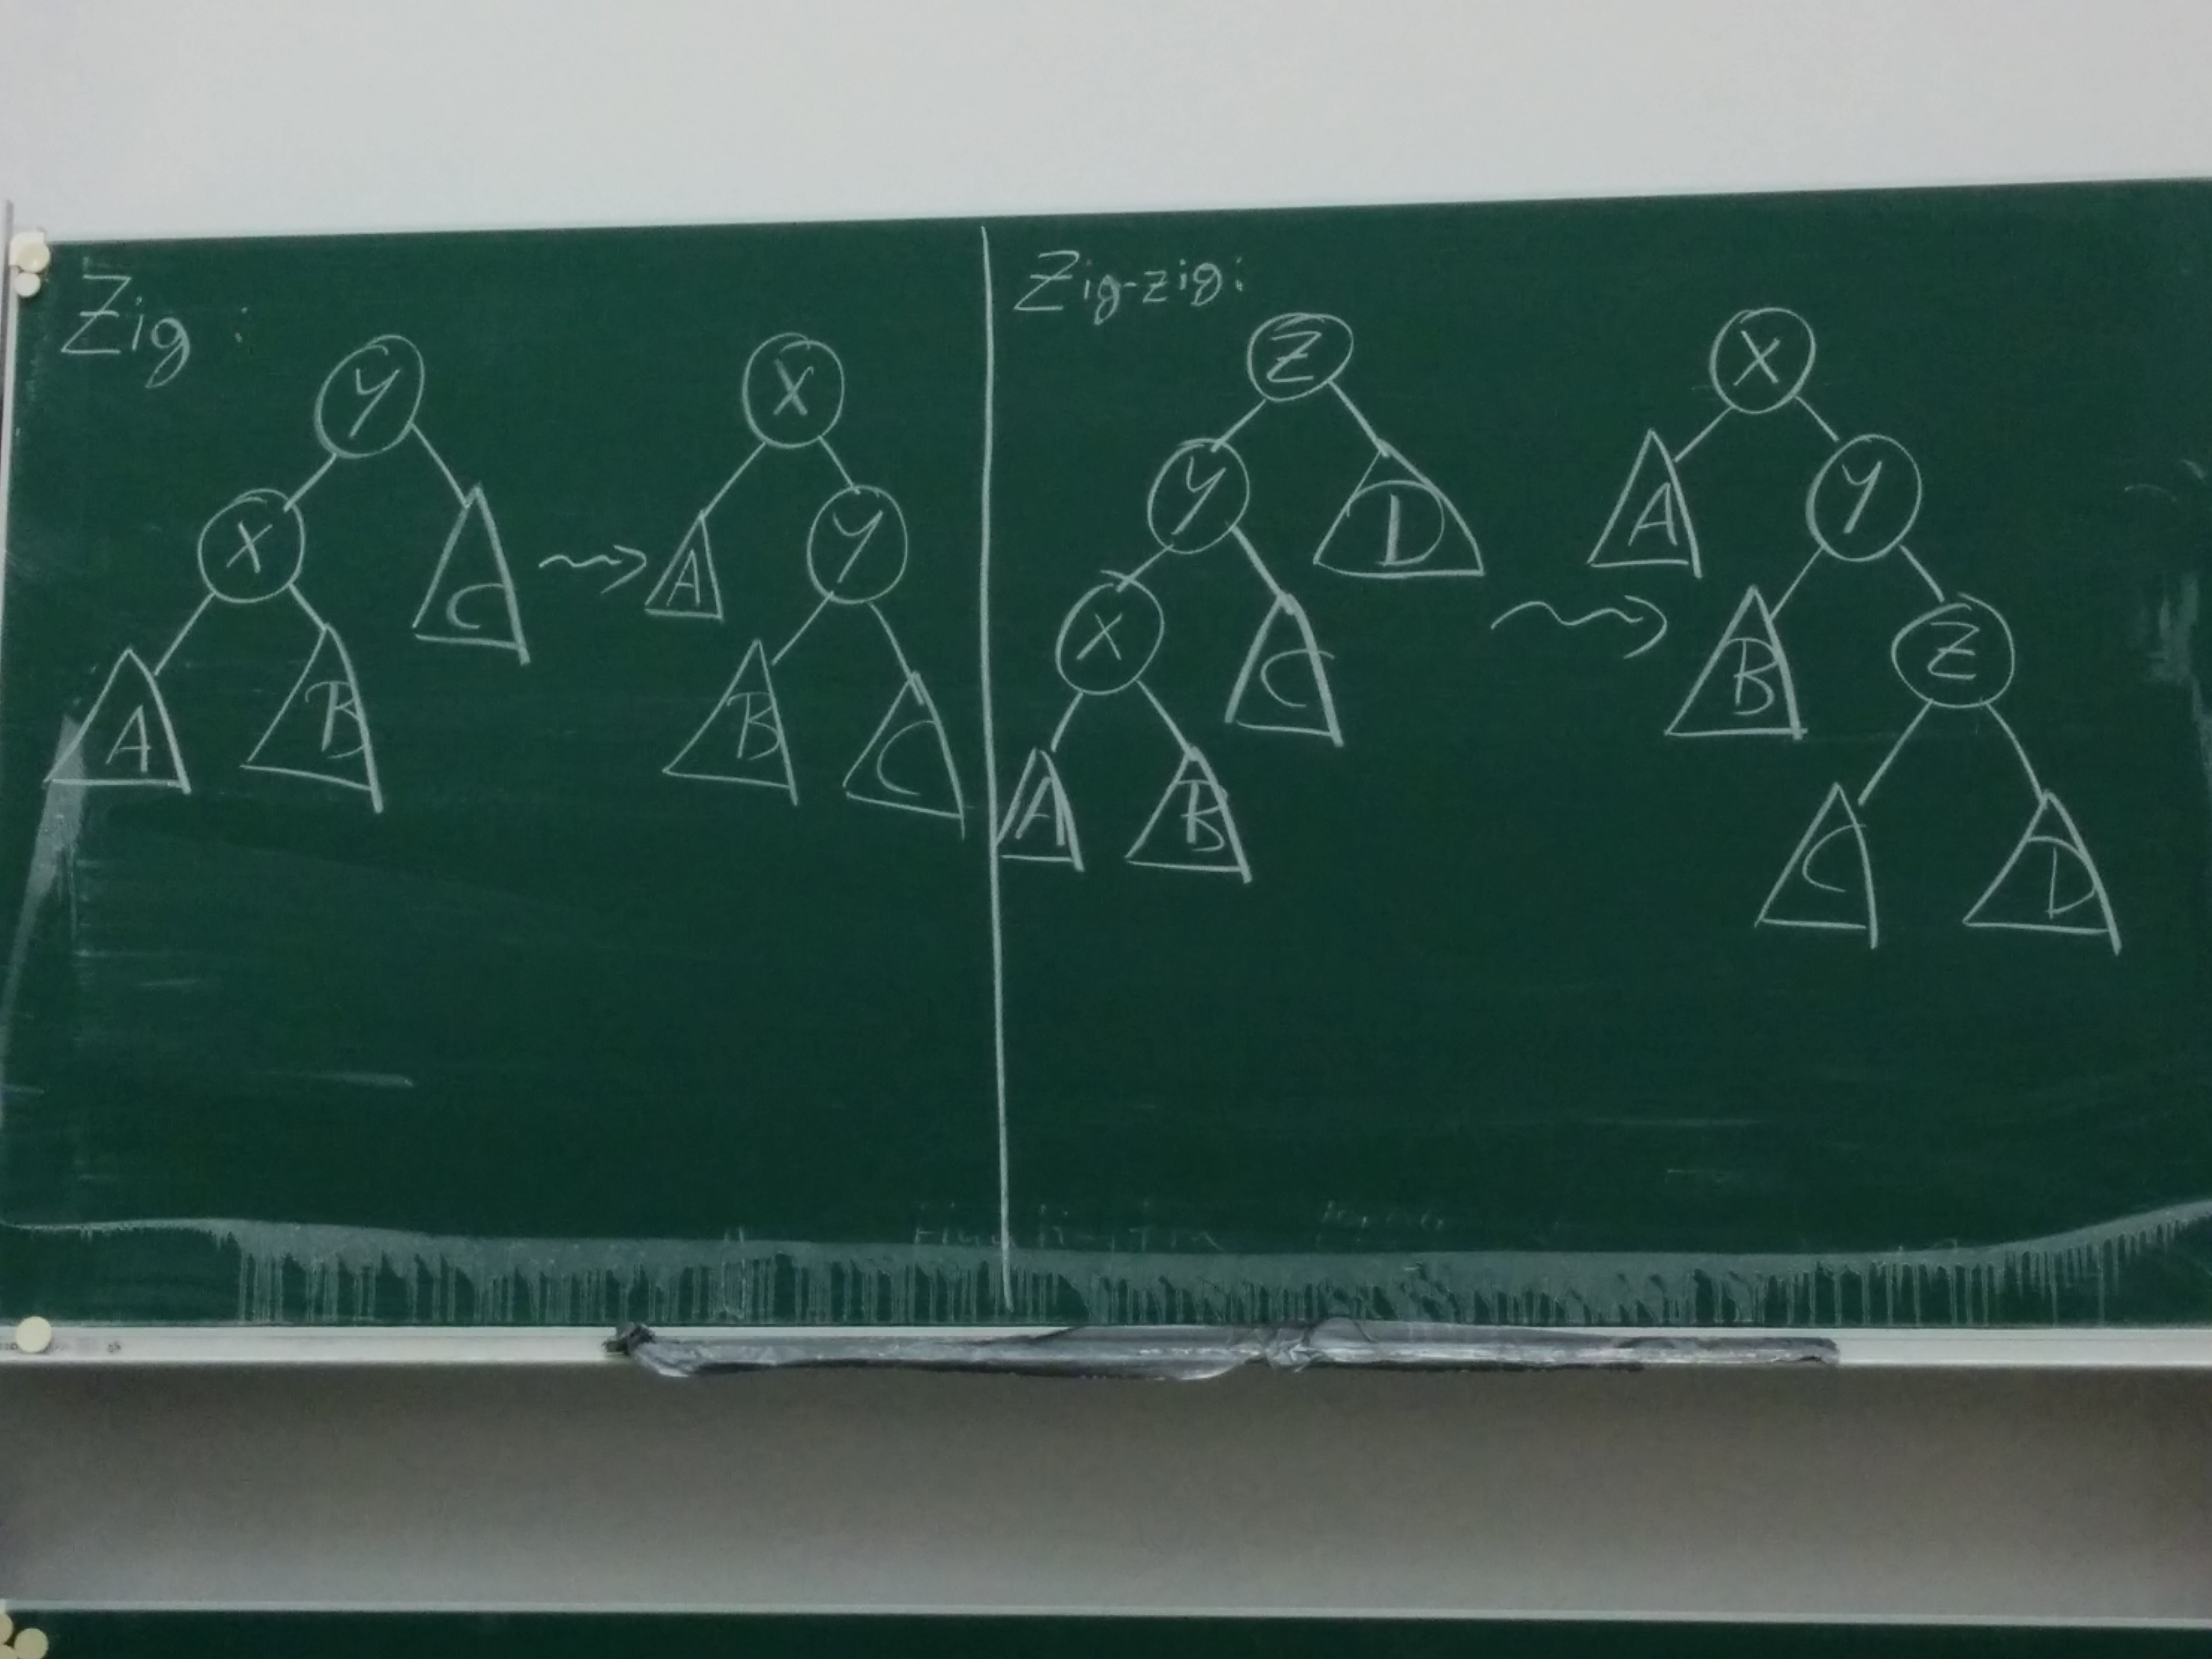
\includegraphics[width=430px]{tree1.jpg}

%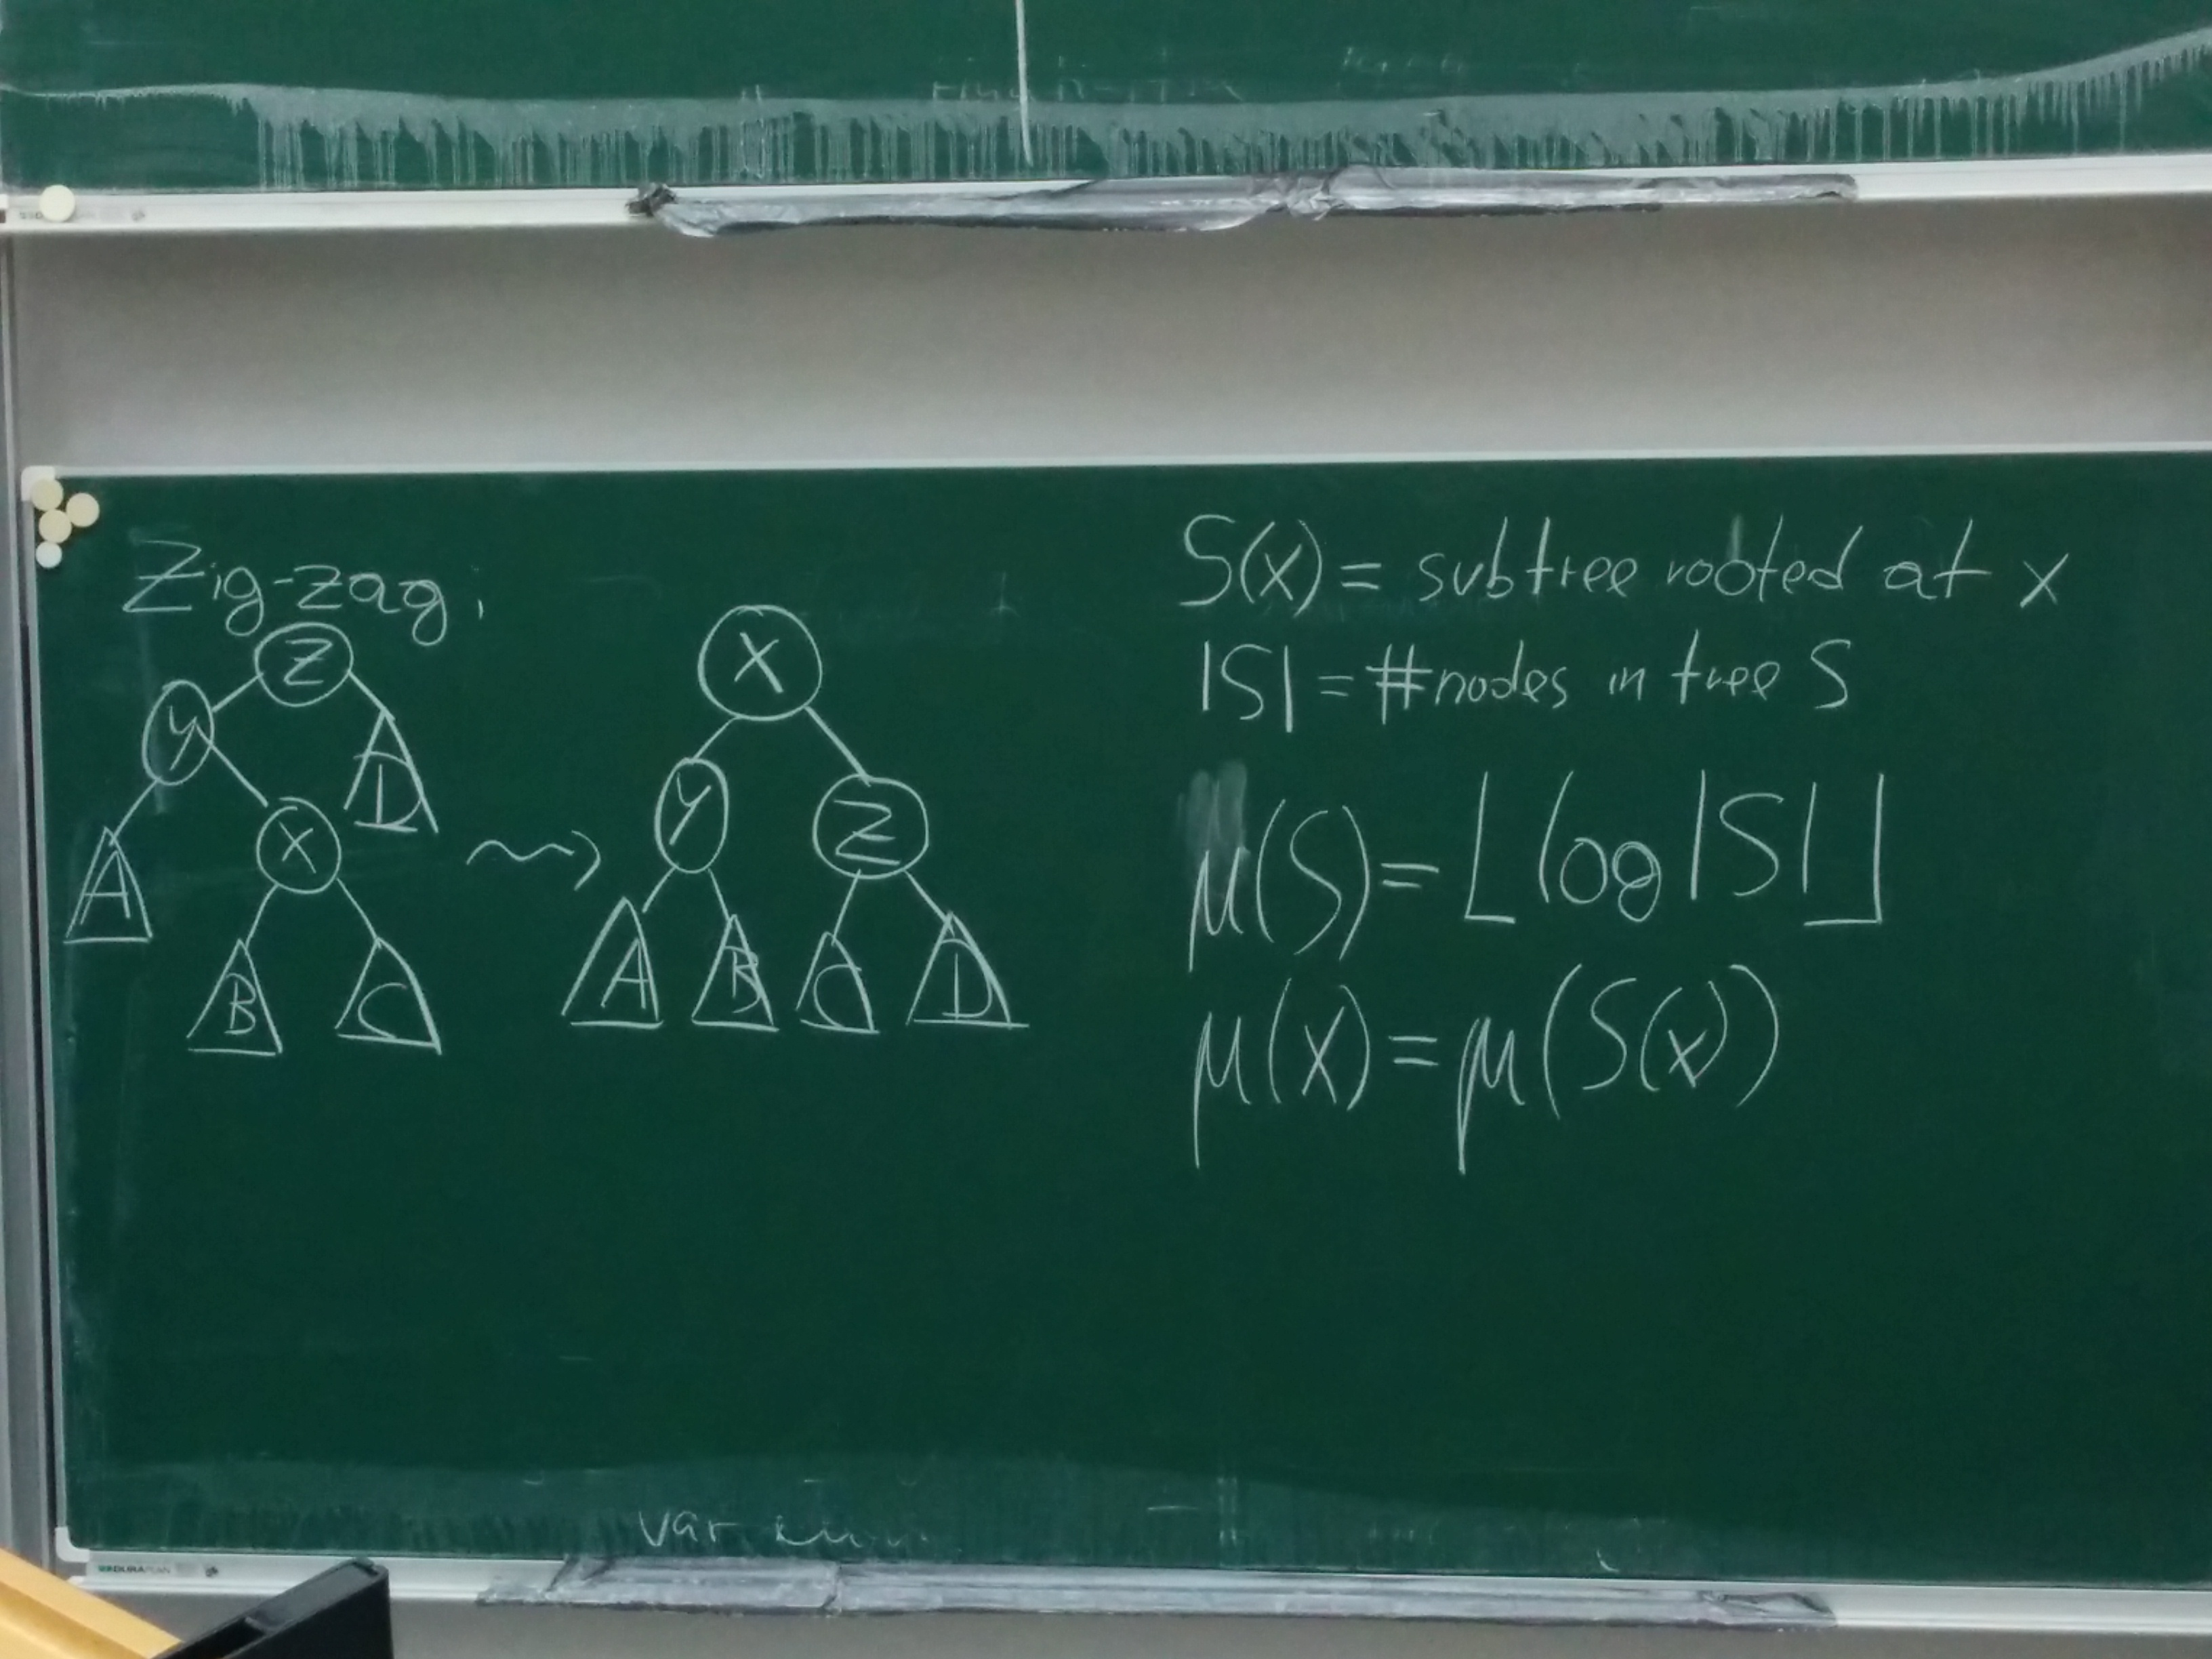
\includegraphics[width=430px]{tree2.jpg}

\begin{mylemma}
Let $x$ be the node that becomes root after a splay operation on tree $T$. We need to spent at most

$$3(\mu(T)-\mu(x)) + 1$$

tokens to pay for all steps and maintain the credit invariant.
\end{mylemma}
\begin{proof}
The cost of finding $x$ is proportional to the cost of rotating $x$ to the root, so we can concentrate on the latter.

For a fixed rotation, let $\mu$ and $\mu'$ denote the weight of a node before and after the rotation. We show:

\begin{enumerate}
\item In a zig-case, we need to pay at most $3(\mu'(x) - \mu(x)) + 1$ tokens.
\item In zig-zig or zig-zag case, we need to pay at most $3(\mu'(x)-\mu(X))$ tokens.
\end{enumerate}

$$[3(\mu'(x)-\mu(x))+3(\mu''(x)-\mu'(x)) + \ldots = 3(\mu(T)-\mu(x))+1] \text{ (telescoping sum)}$$

\paragraph{Proof of (i):} We have that $\mu(y) = \mu'(x)$, and $\mu'(y) \le \mu'(x)$. We have to pay:

\begin{align*}
\underbrace{(\mu'(x) - \mu(x))}_\text{credit inv. for $x$} \quad + \quad \underbrace{(\mu'(y)-\mu(y))}_\text{credit inv. for $y$} \quad + \quad \underbrace{1}_\text{for paying the rotation}  
& \le \mu'(x) -\mu(x) + 1 \\
& \le 3(\mu'(x) - \mu(x)) + 1
\end{align*}

\paragraph{Proof of (ii):} Consider a zig-zag. We need

$$C = \mu'(x) - \mu(x) + \mu'(y) - \mu(y) + \mu'(z) - \mu(z) + 1$$

tokens. Since $\mu'(x) - \mu(z)$, this simplifies to:

\begin{align*}
C & \le \mu'(y) - \mu(x) + \mu'(z) - \mu(y) + 1 \\
& \le \mu'(x) - \mu(x) + \mu'(x) - \mu(x) + 1 \\
& = 2(\mu'(x) - \mu(x)) + 1
\end{align*}

If $\mu(x) - \mu(x) > 0$, this is at most $3(\mu'(x) - \mu(x))$ and we are done. What if $\mu(x) = \mu(x)$? We show that $\mu(x)=\mu(x)$ implies that $C\le 0$, so we have to spend $0 \le 3(\mu'(x)-\mu(x)$.

By contradiction, assume $\mu'(x)=\mu(x)$ and $C\ge 1$. That means $\mu'(x)=\mu(x)$ and $(\mu'(x)+\mu'(y)+\mu'(z) \ge \mu(x)+\mu(y)+\mu(z)$.

Since $\mu(x)=\mu'(x)=\mu(z)$, we have that $\mu(y) = \mu(x) = \mu(z)$. So, the inequality simplifies to

$$\mu'(y) + \mu'(z) \ge 2\mu'(x),$$

which implies $\mu'(x) = \mu'(y) = \mu'(z) = \mu(x) = \mu(y) = \mu(z)$.

Consider $a = |S(x)|$ before rotating, and $b = |S(z)|$ after rotating.

Then $\underbrace{\lfloor \log a \rfloor}_{=\mu(x)} = \underbrace{\lfloor\log a + b + 1\rfloor}_{=\mu'(x)} = \underbrace{\lfloor \log b \rfloor}_{=\mu'(z)}$

For $a \le b$, $\mu'(x) = \lfloor \log a + b + a \rfloor \ge \lfloor \log 2a \rfloor \ge 1 + \lfloor \log a \rfloor > \lfloor \log a \rfloor$.

So $C \le 0$.
\end{proof}

\begin{mytheorem}
For an initially empty splay tree, a sequence of $m$ insertions/removals/searches with $n$ inserts costs $O(m \log n)$.
\end{mytheorem}
\begin{proof}
Every splay step pays $O(\log n)$ tokens to perform all operations. When inserting a node, we have to put $\log n$ tokens on its account for the credit invariant.
\end{proof}

\section{Heaps}

\begin{itemize}
\item Sorted sequences with restricted access patterns.
\item Elements have keys (priorities) as usual
\end{itemize}

A \emph{non-addressable priority queue} $Q$ supports:
\begin{itemize}
\item ${insert}(e, Q)$
\item ${min}(Q)$: return element with smallest key
\item ${delete\_min}(Q)$: remove smallest element
\item ${build}(e_1, \ldots, e_n)$: creates a priorirty queue with elements $e_1, \ldots, e_n$
\end{itemize}

A handle $h$ is a pointer to an element stored in $A$.
An \emph{addressable priorirty queue} $Q$ supports:
\begin{itemize}
\item ${insert}(e, Q)$: returns a handle to inserted element
\item ${remove}(h, Q)$: remove the element pointed by $h$
\item ${min}(Q)$
\item ${delete\_min}(Q)$
\item ${build}(e_1, \ldots, e_n)$
\item ${decrease\_key}(h, k, Q)$: replaces the key of $h$ with $k$ (must be smaller than old key)
\item ${union}(Q_1, Q_2)$: merges the priority queues $Q_1$ and $Q_2$
\end{itemize}

\subsection{Binary Heaps}

\begin{itemize}
\item It is a maximally balanced binary tree
\item Last level is left-aligned
\item One element per node
\item Heap-ordered: key at node $v$ is smaller than all keys in descendants of $v$
\item Can be stored as an array
\end{itemize}

\begin{lstlisting}[mathescape]
${insert}(e, Q)$:
    put $e$ at next free position in node $v$
    sift_up(v)
    
${sift\_up}(v)$:
    $w \gets {parent}(v)$
    if ${key}(v) > {key}(w)$, return
    else
        swap elements of $v$ and $w$
        ${sift\_up}(w)$
\end{lstlisting}

\begin{lstlisting}[mathescape]
${delete\_min}(Q)$:
    swap elements of root and last element in order
    delete last element
    ${sift\_down}({root})$

${sift\_down}(v)$:
    if $v$ is leaf, return
    $w \gets$ smallest child of $v$
    if ${key}(v) < {key}(w)$, return
    else
        swap contents of $v$ and $w$
        ${sift\_down}(w)$
\end{lstlisting}

\paragraph{Build: } Let $e_1, \ldots, e_n$ be the elements of the heap. Put the elements in any order and call ${heapify}({root})$.
\begin{lstlisting}[mathescape]
${heapify}(v)$:
    if $v$ has left child $w$:
        ${heapify}(w)$
    if $v$ has right child $w'$:
        ${heapify}(w')$
    ${sift\_down}(v)$
\end{lstlisting}

\paragraph{Cost: } A ${sift\_down}$ on level $i$ costs not more than $\log n -i$ steps. The total cost is given by:

\begin{align*}
\sum_{i = 0}^{\lfloor \log n \rfloor} 2^i (\log n - i) \\
& = \sum_{j = 0}^{\lfloor \log n \rfloor} 2^i (\log n - j) j \\
& = n \cdot \underbrace{\sum_{j = 0}^{\lfloor \log n \rfloor} \frac{1}{2^j} \cdot j}_{\le 2} \\
& = O(n)
\end{align*}

\begin{align*}
\sum_{j=0}^\infty \frac{j}{2^j} = \sum_{j \ge 1} \frac{j}{2^j} & = \sum_{j \ge 1} \frac{1}{2^j} + \sum_{j \ge 2} \frac{1}{2^j} + \sum_{j \ge 3} \frac{1}{2^j} + \ldots  \\
& = \sum_{j \ge 1} \frac{1}{2^j} + \frac{1}{2} \sum_{j \ge 2} \frac{1}{2^{j-1}} + \frac{1}{4} \sum_{j \ge 3} \frac{1}{2^{j-2}} + \ldots \\
& = \sum_{j \ge 1} \frac{1}{2^j} + \frac{1}{2} \sum_{j \ge 1} \frac{1}{2^j} + \frac{1}{4} \sum_{j \ge 1} \frac{1}{2^j} + \ldots \\
& = \underbrace{\sum_{j \ge 1} \frac{1}{2^j}}_{=1} \left ( 1 + \frac{1}{2} + \frac{1}{4} + \ldots \right ) \\
& \le 2
\end{align*}






\newpage \section{Fibonacci Heaps}

\paragraph{Representation:}

\begin{itemize}
\item Forest of (arbitrary) heap-ordered trees
\item Min-pointer to smallest element ($\implies {min}(Q) = O(1)$)
\item Roots are connected by a linked list, called the \emph{root list}
\end{itemize}

\paragraph{Every node contains:}

\begin{itemize}
\item One element
\item Its rank (= \# children)
\item Pointers to parent, left and right sibling, and to one child
\item A flag (marked or not) used in ${decrease\_key}$.
\end{itemize}

\paragraph{Operations:}

\begin{itemize}
\item ${insert}(e,Q)$: Add new tree with one node $e$ to root list and update the ${min}$ pointer $\implies O(1)$.
\item ${union}(Q_1, Q_2):$ Splice the root lists and update the ${min}$ pointer $\implies O(1)$.
\item ${remove}(h, Q):$ ${decrease\_key}(h, -\infty, Q)$, then, ${delete\_min}(Q)$. 
\end{itemize}

\begin{lstlisting}[mathescape]
${delete\_min(Q)}$
    Delete min-node and add all its children to the root list
    Create and unbounded array $A$ storing handles to roots
    Traverse the root list. Let $v$ be a root and $r$ its rank:
        while($A[r] \neq \bot$):
            Let $w = A[v]$, so ${rank}(v)=r={rank}(w)$.
            Combine $v$ and $w$ into a new tree by making either $v$ a child
            of $w$ or vice versa.
            $A[v] \gets \bot$
            $r \gets r + 1$
        $A[v] \gets V$
    Traverse $A$ once more and find ${min-node}$ to update the pointer
            
\end{lstlisting}

${Decrease\_key}$ can be defined as follows:

\begin{lstlisting}[mathescape]
${decrease\_key(h, k, Q)}$
    Cut subtree at $h$ and make it a new root
    Update its key and update the ${min\_pointer}$. $\implies O(1)?$
\end{lstlisting}

However, this allows too ``wild'' shapes for the trees.



\begin{lstlisting}[mathescape]
Repair (Cascading Cuts):
    When node $v$ is cut, let $w$ be its parent.
    while($w$ is marked):
        Unmark and cut $w$
        $w \gets$ (old) parent of $w$
\end{lstlisting}

\subsection{Amortized Analysis}

\paragraph{Credit Invariant:} Each root holds one token and each marked node holds two tokens.

Let $R$ be the maximal rank of a node in the Fibonacci Heap.

\begin{mylemma}
${decrease\_key}$ needs to pay $O(1)$ credits to perform all its operations and maintain the credit invariant.
\end{mylemma}
\begin{proof}
The methods marks (at most) one element and we can spend the two tokens for this marking. The first cut costs $O(1)$. Any further cut turns a marked node into a root, so one token becomes free and we spend it to pay for the cut.
\end{proof}

\begin{mylemma}
${delete\_min}$ needs to pay $O(R)$ credits to pay for all its operations and to maintain the credit invariant.
\end{mylemma}
\begin{proof}
We need to pay $O(R)$ credits to make the children of min-node roots and give them one token each. The array $A$ has size $O(R)$, and ${delete\_min}$ can pay for initialization.

The running time of the loop is $O(R + \# {combines})$. Each combine turns some root into a non-root, so we can use its token to pay or the combine. Finding the min-pointer costs at most $O(R)$ additional operations.
\end{proof}

It remains to show that $R = O(\log n)$.

\paragraph{Fibonacci Numbers:}
\begin{itemize}
\item $F_0 = 0, F_1 = 1, \forall i \ge 2, FI = F_{i-1} + F_{i - 1}$
\item 0,1, 1,2,3,5,8,13,21, \ldots
\end{itemize}

\begin{mylemma}
$F_{i + 2} \ge \left ( \frac{1 + \sqrt{5}}{2} \right )^i \ge 1.618^i$ (homework).
\end{mylemma}

\begin{mylemma}
Let $v$ be a node of rank $i$. Then, the subtree rooted at $v$ has at least $F_{i+2}$ nodes. In particular, if the FH has $n$ nodes, each rank is bounded by $1.4404 \log n$.
\end{mylemma}
\begin{proof}
Let $v$ be a node of rank $i$. Let $w_1, \ldots, w_i$ be its children, sorted in order when they became children of $v$. For $w_j, 1 \le j \le i$, $w_j$ became child of $v$ through a combine in ${delete\_min}$. So, the rank of $w_j$ at that time was at least $j - 1$, because $w_1, \ldots, w_{j-1}$ were children of $v$ and combine only merges roots of same rank. Because $w_j$ has lost at most one child since then, ${rank}(w_j) \ge j-2$.

Let $S_i$ be the minimum number of nodes in a subtree with a root of rank $i$. We have $S_0 = 1, S_i \ge 2$ and $\forall i \ge 2, S_i \ge 2 + S_0 + S_1 + \ldots + S_{i-2}$.

We have that $S_i \ge F_{i+2}$ (homework).

For the second claim, for any ode of tank $i$, we have $F_{n+2} \le n \iff 1.618^n \le n \iff i \le 1.4404 \log n$.
\end{proof}

\section{Union-find}

We want to represent a collection of \emph{disjoint} sets $S_1, \ldots, S_k$. Each set $S_i$ has a representative $r_i \in S_i$. Our data structure suports:

\begin{itemize}
\item ${make\_set}(x):$ Create a new set $\{x\}$
\item ${union}(x, y):$ Combine $S_i$ and $S_j$, where $x \in S_i$ and $y \in S_j$, into a new set $S_i \cup S_j$ and pick some element of the union as representative.
\item ${find}(x):$ return the representative of the set containing $x$
\end{itemize}
 
\paragraph{Application:} Find the connected components of a graph $\implies$ minimum spanning tree.

\paragraph{Representation: }
\begin{itemize}
\item Forest of (arbitrary) trees, one per set
\item One element per node. Root contains the representative.
\item Only pointer to the parent. Root points to itself.
\end{itemize}

Naive implementation of ${make\_set}$, ${union}$, ${find}$ is clear. Efficiency? Bad, because trees can degenerate.

\paragraph{Optimization 1: } ``Union by ranks''. Merge the less deep tree into the deeper tree.


\section{Graph Algorithms}

\subsection{Connectivity}

We have a directed graph $G=(V,E)$, \emph{simple} (no loops or multi edges).

$$n = |V|, m = |E|$$

\paragraph{(Directed) Path of length $k$}

\paragraph{(Directed) Cycle of length $k+1$: } Directed path of length $k$ + find edge $(v_{k+1}, v_1)$.

\paragraph{Simple path, simple cycle: } No vertex appears twice on the path/cycle.

\begin{itemize}
\item Graph $G=(V, E)$ is \emph{strongly connected} if it has a $(v,u)$-path and $(u,v)$ path for all $v,w \in V$.

\item Undirected graph $G$ is $k$-connected ($k$-vertex connected) if removal of at most $k-1$ vertices (and all incident edges) keeps the graph connected. $k$-edge connected similar, but for edge removal.

\item An inclusion-maximal strongly connected subgraph is a strongly connected component. Same for $k$-connected and $k$-edge-connected. \emph{Intuitively, it cannot be extended with more vertices/edges and maintain the same property.}
\end{itemize}

\subsection{DFS Framework}

\begin{lstlisting}[mathescape]
Input: Graph directed or indirected, $G=(V,E)$
Data Structure:
    Stack S (for vertices on the DFS path)
    Vertex array "incoming" (for first incoming edge)
    Vertex & edge markings

for each $s \in V$ do:
    mark S, set incoming[s] $\gets$ nil, push $s \rightarrow S$
    root(S)
    
    while S is not empty do:
        $v \gets top(S)$
        if $\exists$ unmarked $e = (v,w) \in E$ then
            mark $e$
            if $w$ is unmarked:
                mark $w$, set incoming[$w$] $\gets$ e, push $w$
                traverse(v,e,w)
        else:
            $w \gets pop(S)$
            backtrack(w, incoming[w], top(S))
\end{lstlisting}

Sequence in which vertices are discovered/marked: $v_1, v_2, \ldots, v_n$.
\begin{itemize}
\item \emph{DFS-number} of $v_i$ as $DFS(v_i) = i$.
\item \emph{DFS-number} of $(v,w$) is $DFS((v,w)) = DFS(v)$.
\item \emph{DFS-order} $\preceq$ on $V$ or $E$ by:
\end{itemize}

$$DFS(p) \le DFS(q) \iff p \preceq q$$

$$DFS(p) < DFS(q) \iff p \prec q$$

\paragraph{Edge Classes: } If $(v,w)$ is marked, it becomes a
\begin{itemize}
\item \emph{tree edge} if $w$ is unmarked
\item \emph{back edge} if $w$ is marked, $w \preceq v, w \in S$
\item \emph{cross edge} if $w$ is marked, .......
\end{itemize}

\subsection{Undirected DFS}

\begin{itemize}
\item Edges are traversed independently of direction.
\item Replace the check of $\exists$ unmarked $e=(v,w) \in E$ with: $e=(v,w) \in E$ or $e=(w,v) \in E$.
\item In undirected DFS, there are no cross and no forward edges (homework!).
\end{itemize}

\subsection{Connected Components}

\begin{lstlisting}[mathescape]
root(s):
    $c \gets s$. component[S] $\gets c$

traverse(v,e,w):
    component[e] $\gets c$, component[w] $\gets c$.
\end{lstlisting}

\begin{itemize}
\item Component is represented by first discovered vertex.
\item Output: Array ``component'', pointing to representing vertex of the component
\item Requires $O(n+m)$ time, $O(n+m)$ space.
\end{itemize}

\subsection{2-connected Components}

\begin{mylemma}
For an undirected graph $h$, edges $e, e' \in E$ are in a 2-connected component if, and only if, there is a simple undirected cycle that contains both $e$ and $e'$. The set of 2-connected components is a partition of the $E$.
\end{mylemma}
\begin{proof}
If a cycle exists, then $e$ and $e'$ are in a 2-connected component.

Subdivide $e$ and $e'$ each with a new vertex. Component is still 2-connected.
Existence of a simple cycle follows from Menger's Theorem.
\end{proof}

\begin{mytheorem}[Menger's Theorem]
In a 2-connected undirected graph with at least 2 edges there are two vertex-disjoint paths between every pair of vertices.
\end{mytheorem}

\begin{proof}[Proof for partition statement]
For the partition statement, assume by contradiction $e$ is in two 2-connected components. There is a simple undirected cycle between $e'$ in one component and $e''$ in the other component. 
There are simple cycles, and they exist for every pair in the union of components. But components must be inclusion-maximal. Contradiction.
\end{proof}

\subsection{Undirected DFS for 2-connected components}

\begin{itemize}
\item Stack $S_E$ for edges in unfinished (or open) components
\item Stack $C$ for open components (represented by first edge)
\item Output: Array ``component'' pointing to representing edge
\end{itemize}

\begin{lstlisting}[mathescape]
traverse(v,e,w):
    push $e \rightarrow S_E$
    if $e$ is free edge then push $e \rightarrow C$
    if $e$ is back edge then:
        while $w \prec$ top(c) do:
            pop(c)

backtrack(w,e,v):
    if $e = top(c)$ and $e \neq nil$ then:
        pop(c)
        repeat
            $e' \gets pop(S_E)$
            component[$e'$] $\gets e$
        until $e = e'$.
\end{lstlisting}


\end{document}